% Licensed to the Apache Software Foundation (ASF) under one
% or more contributor license agreements.  See the NOTICE file
% distributed with this work for additional information
% regarding copyright ownership.  The ASF licenses this file
% to you under the Apache License, Version 2.0 (the
% "License"); you may not use this file except in compliance
% with the License.  You may obtain a copy of the License at
%
%     http://www.apache.org/licenses/LICENSE-2.0
%
% Unless required by applicable law or agreed to in writing, software
% distributed under the License is distributed on an "AS IS" BASIS,
% WITHOUT WARRANTIES OR CONDITIONS OF ANY KIND, either express or implied.
% See the License for the specific language governing permissions and
% limitations under the License.
\documentclass{article}
\usepackage[pdftex]{hyperref}
\usepackage[pdftex]{graphicx}

\title{Winning a 60 Second Dash with a Yellow Elephant}
\author{\href{http://people.apache.org/~omalley}{Owen O'Malley} and 
        \href{http://people.apache.org/~acmurthy}{Arun C. Murthy}\\
\href{http://www.yahoo.com/}{Yahoo!}\\
owen@yahoo-inc.com and acm@yahoo-inc.com}
\date{April 2009}
\begin{document}
\maketitle
\href{http://hadoop.apache.org/core}{Apache Hadoop} is a open source
software framework that dramatically simplifies writing distributed
data intensive applications. It provides a distributed file system,
which is modeled after the Google File System\cite{gfs}, and a
map/reduce\cite{mapreduce} implementation that manages distributed
computation. Jim Gray defined a benchmark to compare large sorting
programs. Since the core of map/reduce is a distributed sort, most of
the custom code is glue to get the desired behavior.

\section{Benchmark Rules}

Jim's Gray's sort benchmark consists of a set of many related
benchmarks, each with their own rules. All of the sort benchmarks
measure the time to sort different numbers of 100 byte records. The
first 10 bytes of each record is the key and the rest is the
value. The \textbf{minute sort} must finish end to end in less than a
minute. The \textbf{Gray sort} must sort more than 100 terabytes and
must run for at least an hour.

\begin{itemize}
\item The input data must precisely match the data generated by the C
  data generator.
\item The input must not be in the operating system's file
  cache when the job starts.. Under Linux, this requires using the memory for something
  else between sorting runs.
\item The input and output data must not be compressed.
\item The output must not overwrite the input.
\item The output must be synced to disk.
\item The 128 bit sum of the crc32's of each key/value pair must be
  calculated for the input and output. Naturally, they must be
  identical.
\item The output may be divided into multiple output files, but it
  must be totally ordered (simply concatenating the output files must
  produce the completely sorted output).
\item Starting and distributing the application to the cluster must be
  included in the execution time.
\item Any sampling must be included in the execution time.
\end{itemize}

\section{Hadoop implementation}

We extended the programs from last year to create and manipulate the
new binary format and match the new rules. There are now 4 Hadoop
map/reduce applications to support the benchmark:
\begin{enumerate}
\item \textbf{TeraGen} is a map/reduce program to generate the data.
\item \textbf{TeraSort} samples the input data and uses map/reduce to
  sort the data into a total order.
\item \textbf{TeraSum} is a map/reduce program computes the 128 bit
  sum of the crc32 of each key/value pair.
\item \textbf{TeraValidate} is a map/reduce program that validates the
  output is sorted and computes the sum of the checksums as TeraSum.
\end{enumerate}
The update to the terasort programs will be checked in as
\href{http://issues.apache.org/jira/browse/HADOOP-5716}{HADOOP-5716}.

\textbf{TeraGen} generates input data for the sort that is byte for byte
equivalent to the C version that was released in March of 2009,
including specific keys and values. It divides the desired number of
rows by the desired number of tasks and assigns ranges of rows to each
map. The map jumps the random number generator to the correct value
for the first row and generates the following rows.

\textbf{TeraSort} is a standard map/reduce sort, except for a custom
partitioner that ensures that all of the keys in reduce $N$ are after
all of the keys in reduce $N-1$. This is a requirement of the contest
so that the output of the sort is totally ordered, even if it is
divided up by reduce.

We wrote an input and output format, used by all 4 applications to
read and write the files in the new format.

\textbf{TeraSum} computes the 128 bit sum of the CRC32 of each
key/value pair. Each map computes the sum of its input and emits a
single 128 bit sum. There is a single reduce that adds the sums from
each map. We used this program on the input directory to calculate the
sum of the checksums of each key/value pair to check the correctness
of the output of the sort. We also used TeraSum on a distinct dataset
that was larger than the total RAM in the cluster to flush the Linux
file cache between runs of the small (500 GB and 1TB) sorts.

\textbf{TeraValidate} ensures that the output is globally sorted. It
creates one map per file in the output directory and each map
ensures that each key is less than or equal to the previous one. The
map also generates records with the first and last keys of the file
and the reduce ensures that the first key of file $i$ is greater that
the last key of file $i-1$. Any problems are reported as output of the
reduce with the keys that are out of order. Additionally, TeraValidate
calculates the sum of checksums of the output directory.

\section{Hardware and Operating System}

We ran our benchmarks on Yahoo's Hammer cluster. Hammer's hardware is
very similar to the hardware that we used in last year's terabyte
sort. The hardware and operating system details are:

\begin{itemize}
\item approximately 3800 nodes (in such a large cluster, nodes are
  always down)
\item 2 quad core Xeons @ 2.5ghz per node
\item 4 SATA disks per node
\item 8G RAM per node (upgraded to 16GB before the petabyte sort)
\item 1 gigabit ethernet on each node
\item 40 nodes per rack
\item 8 gigabit ethernet uplinks from each rack to the core
\item Red Hat Enterprise Linux Server Release 5.1 (kernel 2.6.18)
\item Sun Java JDK (1.6.0\_05-b13 and 1.6.0\_13-b03) (32 and 64 bit)
\end{itemize}

We hit a JVM bug in 1.6.0\_05-b13 on the larger sorts (100TB and 1PB)
and switched over to the later JVM, which resolved the issue. For the
larger sorts, we used 64 bit JVMs for the Name Node and Job Tracker.

\section{Software and Configuration}

The version of Hadoop we used was a private branch of trunk that was
started in January 2009, which is after the 0.20 branch was feature
frozen. We used git to manage our branch and it allowed us to easily
coordinate our work, track our changes, and resynchronize with the
current Hadoop trunk.

The changes include:

\begin{enumerate}

\item Updated the terasort example in the Hadoop code base to match
  the dataset defined by the rule changes in the benchmark from March
  of 2009.
  (\href{http://issues.apache.org/jira/browse/HADOOP-5716}{HADOOP-5716})

\item We reimplemented the reducer side of Hadoop's shuffle. The
  redesign improved the performance of the shuffle and removed
  bottlenecks and over-throttling. It also made the code more
  maintainable and understandable by breaking a 3000 line Java file
  into multiple classes with a clean set of interfaces.
  (\href{http://issues.apache.org/jira/browse/HADOOP-5223}{HADOOP-5223})

\item The new shuffle also fetches multiple map outputs from the same
  node over each connection rather than one at a time. Fetching
  multiple map outputs at the same time avoids connection setup costs
  and also avoids the round trip while the server responds to the request.
  (\href{http://issues.apache.org/jira/browse/HADOOP-1338}{HADOOP-1338})
  
\item Allowed configuring timeouts on the shuffle connections and we
  shortened them for the small sorts. We observed cases where the
  connections for the shuffle would hang until the timeout, which made
  low latency jobs impossibly long.
  (\href{http://issues.apache.org/jira/browse/HADOOP-5789}{HADOOP-5789})

\item Set TCP no-delay and more frequent pings between the Task and
  the Task Tracker to reduce latency in detecting problems.
  (\href{http://issues.apache.org/jira/browse/HADOOP-5788}{HADOOP-5788})

\item We added some protection code to detect incorrect data being
  transmitted in the shuffle from causing the reduce to fail. It
  appears this is either a JVM NIO bug or Jetty bug that likely
  affects 0.20 and trunk under heavy load.
  (\href{http://issues.apache.org/jira/browse/HADOOP-5783}{HADOOP-5783})

\item We used LZO compression on the map outputs. On the new dataset, LZO
  compresses down to 45\% of the original size. By comparison, the
  dataset from last year compresses to 20\% of the original size. Last
  year, the shuffle would run out of direct buffers if we used
  compression on the map outputs.

\item We implemented memory to memory merges in the reduce during the
  shuffle to combine the map outputs in memory before we finish the
  shuffle, thereby reducing the work needed when the reduce is
  running.

\item We multi-threaded the sampling code that read the input set to
  find the partition points between the reduces. We also wrote a
  simple partitioner that assumes the keys are evenly
  distributed. Since the new dataset does not require sampling, the
  simple partitioner produces very even partitions.
  (\href{http://issues.apache.org/jira/browse/HADOOP-4946}{HADOOP-4946})

\item On the smaller clusters, we configured the system with faster
  heartbeat cycles from the Task Trackers to the Job Tracker (it
  defaults to 10 secs / 1000 nodes, but we made it configurable and
  brought it down to 2 seconds/1000 nodes to provide lower latency)
  (\href{http://issues.apache.org/jira/browse/HADOOP-5784}{HADOOP-5784})

\item Typically the Job Tracker assigns tasks to Task Trackers on a
  first come first served basis. This greedy assignment of tasks did
  not lead to good data locality. However, by taking a global view and
  placing all of the map tasks at once, the system achieves much better
  locality. Rather than implement global scheduling for all of Hadoop,
  which would be much harder, we implemented a global scheduler for
  the terasort example in the input format. Basically, the input
  format computes the splits and assigns work to the nodes that have
  the fewest blocks first. For a node that has more blocks
  than map slots, it picks the block that have the fewest remaining
  locations left. This greedy global algorithm seems to get very good
  locality. The input format would schedule the maps and then change
  the input split descriptions to only have a single location instead
  of the original 3. This increased task locality by 40\% or so over
  the greedy scheduler.

\item Hadoop 0.20 added setup and cleanup tasks. Since they are not
  required for the sort benchmarks, we allow them to be disabled to
  reduce the latency of starting and stopping the job.
  (\href{http://issues.apache.org/jira/browse/HADOOP-5785}{HADOOP-5785})

\item We discovered a performance problem where in some contexts the
  cost of using the JNI-based CRC32 was very high. By implementing it
  in pure Java, the average case is a little slower, but the worst
  case is much better.
  (\href{http://issues.apache.org/jira/browse/HADOOP-5598}{HADOOP-5598})

\item We found and removed some hard-coded wait loops from the
  framework that don't matter for large jobs, but can seriously slow
  down low latency jobs.

\item Allowed setting the logging level for the tasks, so that we
  could cut down on logging. When running for "real" we configure the
  logging level to WARN instead of the default INFO. Reducing the
  amount of logging has a huge impact on the performance of the
  system, but obviously makes debugging and analysis much harder.
  (\href{http://issues.apache.org/jira/browse/HADOOP-5786}{HADOOP-5786})

\item One optimization that we didn't finish is to optimize the job
  planning code. Currently, it uses an RPC to the Name Node for each
  input file, which we have observed taking a substantial amount of
  time. For the terabyte sort, our investigations show that we
  could save about 4 seconds out of the 8 that were spent on setting
  up the job.
  (\href{http://issues.apache.org/jira/browse/HADOOP-5795}{HADOOP-5795})

\end{enumerate}

\section{Results}

Hadoop has made a lot of progress in the last year and we were able to
run much lower latency jobs as well as much larger jobs. Note that in
any large cluster and distributed application, there are a lot of
moving pieces and thus we have seen a wide variation in execution
times. As Hadoop evolves and becomes more graceful in the presence of
hardware degradation and failure, this variation should smooth
out. The best times for each of the listed sort sizes were:
\\

\begin{tabular}{| c | c | c | c | c | c |}
\hline
Bytes & Nodes & Maps & Reduces & Replication & Time \\
\hline
$5*10^{11}$ & 1406 & 8000 & 2600 & 1 & 59 seconds \\
$10^{12}$ & 1460 & 8000 & 2700 & 1 & 62 seconds \\
$10^{14}$ & 3452 & 190,000 & 10,000 & 2 & 173 minutes \\
$10^{15}$ & 3658 & 80,000 & 20,000 & 2 & 975 minutes \\
\hline
\end{tabular}\\

Within the rules for the 2009 Gray sort, our 500 GB sort set a new
record for the minute sort and the 1PB sort set a new record of 1.03
TB/minute. The 62 second terabyte sort would have set a new record,
but the terabyte benchmark that we won last year has been
retired. (Clearly the minute sort and terabyte sort are rapidly
converging, and thus it is not a loss.)  One piece of trivia is that
only the petabyte dataset had any duplicate keys (40 of them).

Because the smaller sorts needed lower latency and faster network, we
only used part of the cluster for those runs. In particular, instead
of our normal 5:1 over subscription between racks, we limited it to 16
nodes in each rack for a 2:1 over subscription. The smaller runs can
also use output replication of 1, because they only take minutes to
run and run on smaller clusters, the likelihood of a node failing is
fairly low. On the larger runs, failure is expected and thus
replication of 2 is required. HDFS protects against data loss during
rack failure by writing the second replica on a different rack and
thus writing the second replica is relatively slow.

We've included the timelines for the jobs counting from the job
submission at the Job Tracker. The diagrams show the number of tasks
running at each point in time. While maps only have a single phase,
the reduces have three: \textbf{shuffle}, \textbf{merge}, and
\textbf{reduce}. The shuffle is the transfer of the data from the
maps. Merge doesn't happen in these benchmarks, because none of the
reduces need multiple levels of merges. Finally, the reduce phase is
where the final merge and writing to HDFS happens. I've also included
a category named \textbf{waste} that represents task attempts that
were running, but ended up either failing, or being killed (often as
speculatively executed task attempts). The job logs and configuration
for the four runs, which are the raw data for the charts, are
available on
\href{http://people.apache.org/~omalley/tera-2009/}{http://people.apache.org/~omalley/tera-2009/}.

If you compare this years charts to last year's, you'll notice that
tasks are launching much faster now. Last year we only launched one
task per heartbeat, so it took 40 seconds to get all of the tasks
launched. Now, Hadoop will fill up a Task Tracker in a single
heartbeat. Reducing that job launch overhead is very important
for getting runs under a minute.

As with last year, we ran with significantly larger tasks than the
defaults for Hadoop. Even with the new more aggressive shuffle,
minimizing the number of transfers (maps * reduces) is very important
to the performance of the job. Notice that in the petabyte sort, each
map is processing 15 GB instead of the default 128 MB and each reduce
is handling 50 GB. When we ran the petabyte with more typical values
1.5 GB / map, it took 40 hours to finish. Therefore, to increase
throughput, it makes sense to consider increasing the default block
size, which translates into the default map size, to at least up to 1
GB.

\section{Comments on the Rule Changes}

The group that runs the Gray Sort Benchmark made very substantial
changes to the rules this year. The changes were not announced; but
rather appeared on the website in March. We feel that it was too late
to make rule changes and that the benchmark should have been changed
next year. We'd also like to point out that while most of the changes to
the data generator were positive, it was a poor choice to remove the
skewed distribution of the keys. The previously skewed distribution
required sampling of the input to pick good partition points between
the reduces. The current dataset picks keys so completely random that
sampling is counter productive and yields even less distributions between the
reduces.

\bibliographystyle{abbrv}
\bibliography{tera}

\begin{figure}[!p]
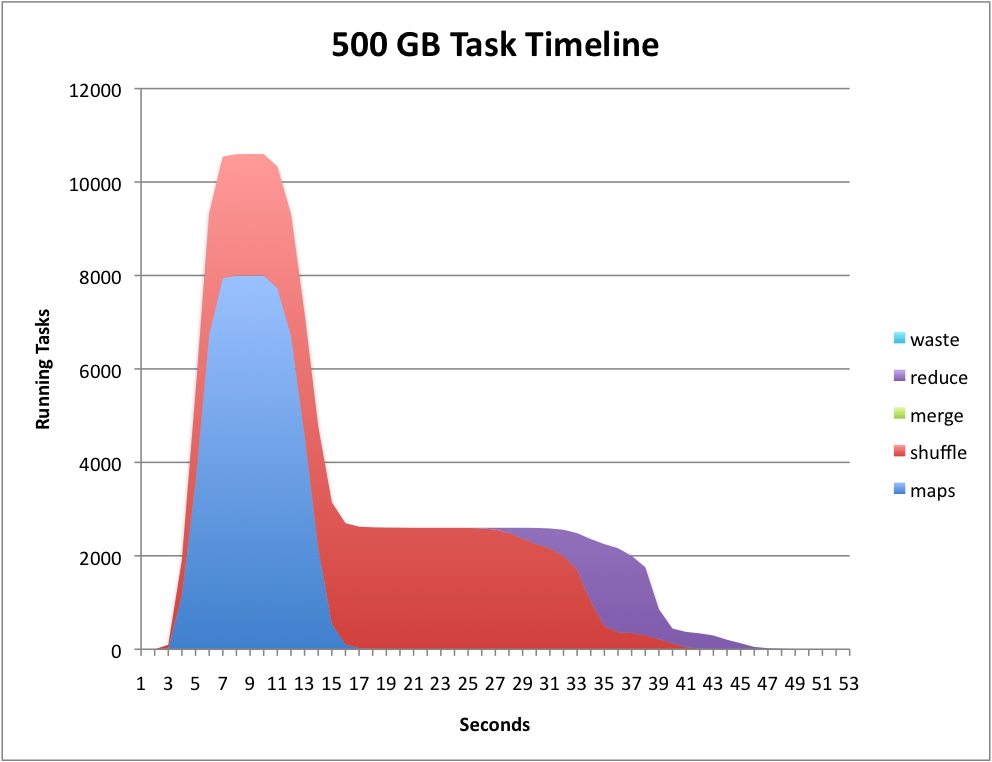
\includegraphics[width=4.21in]{500GBTaskTime.png}
\caption{500 GB sort tasks across time}\label{500GbTimeline}
\end{figure} 

\begin{figure}[!p]
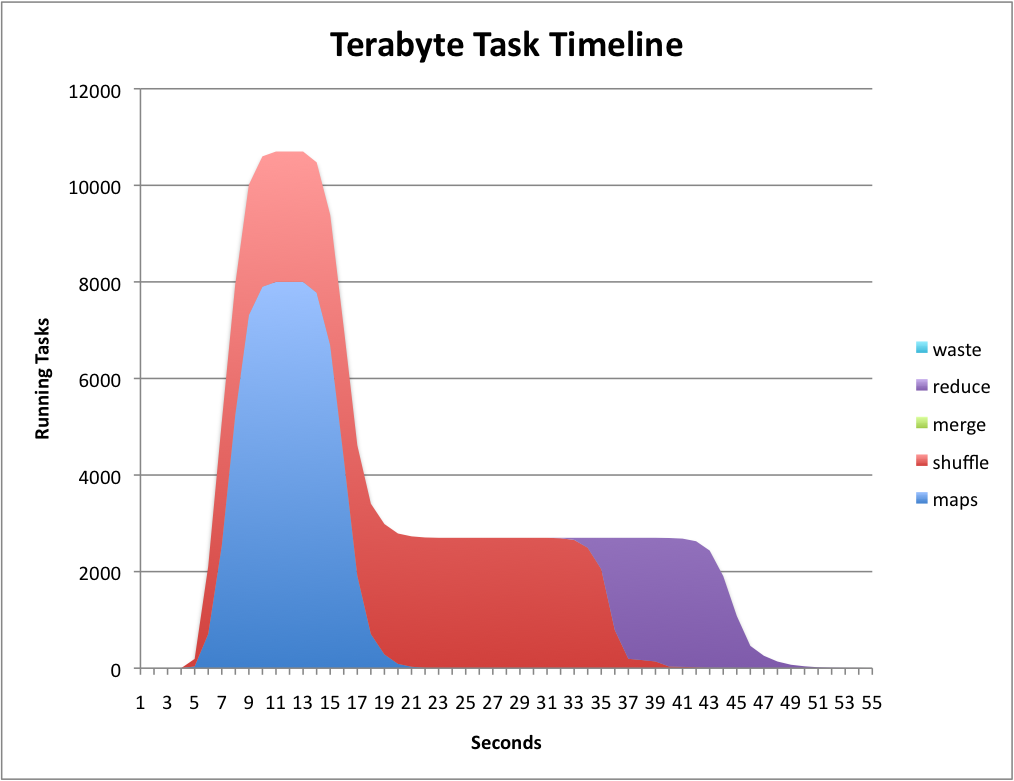
\includegraphics[width=4.5in]{1TBTaskTime.png}
\caption{1 TB sort tasks across time}\label{1TbTimeline}
\end{figure} 

\begin{figure}[!p]
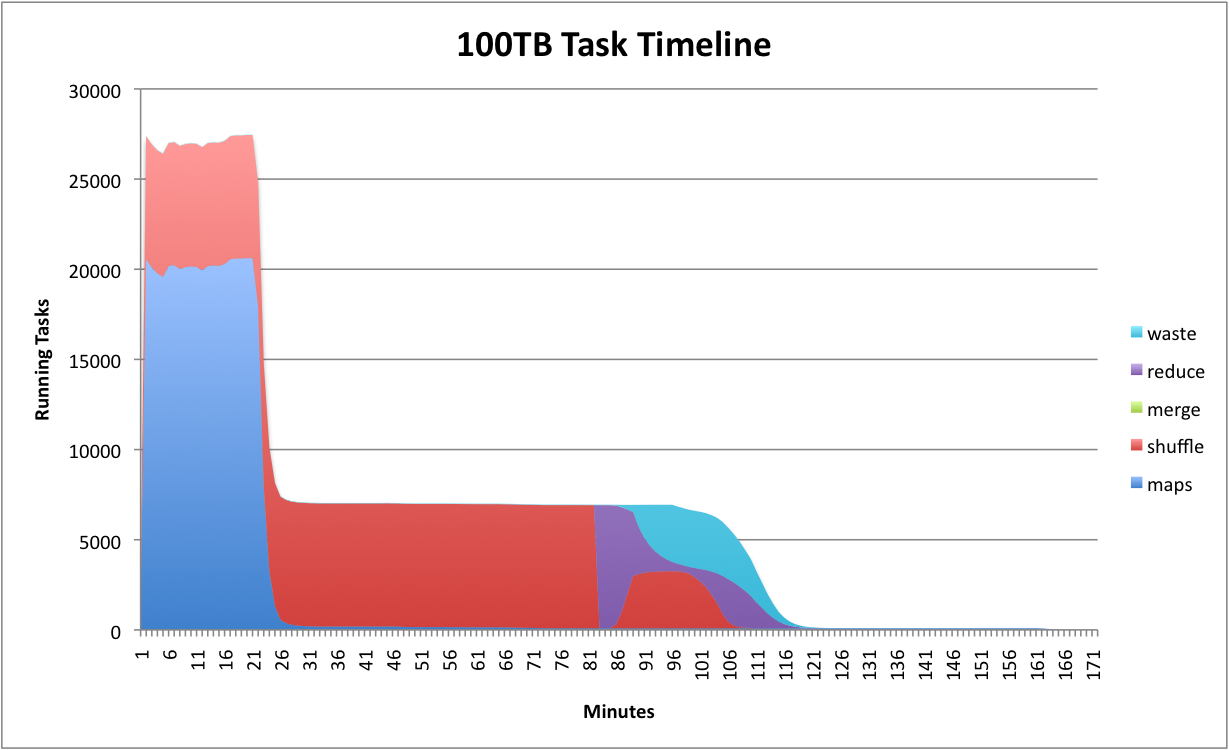
\includegraphics[width=4.5in]{100TBTaskTime.png}
\caption{100 TB sort tasks across time}\label{100TbTimeline}
\end{figure} 

\begin{figure}[!p]
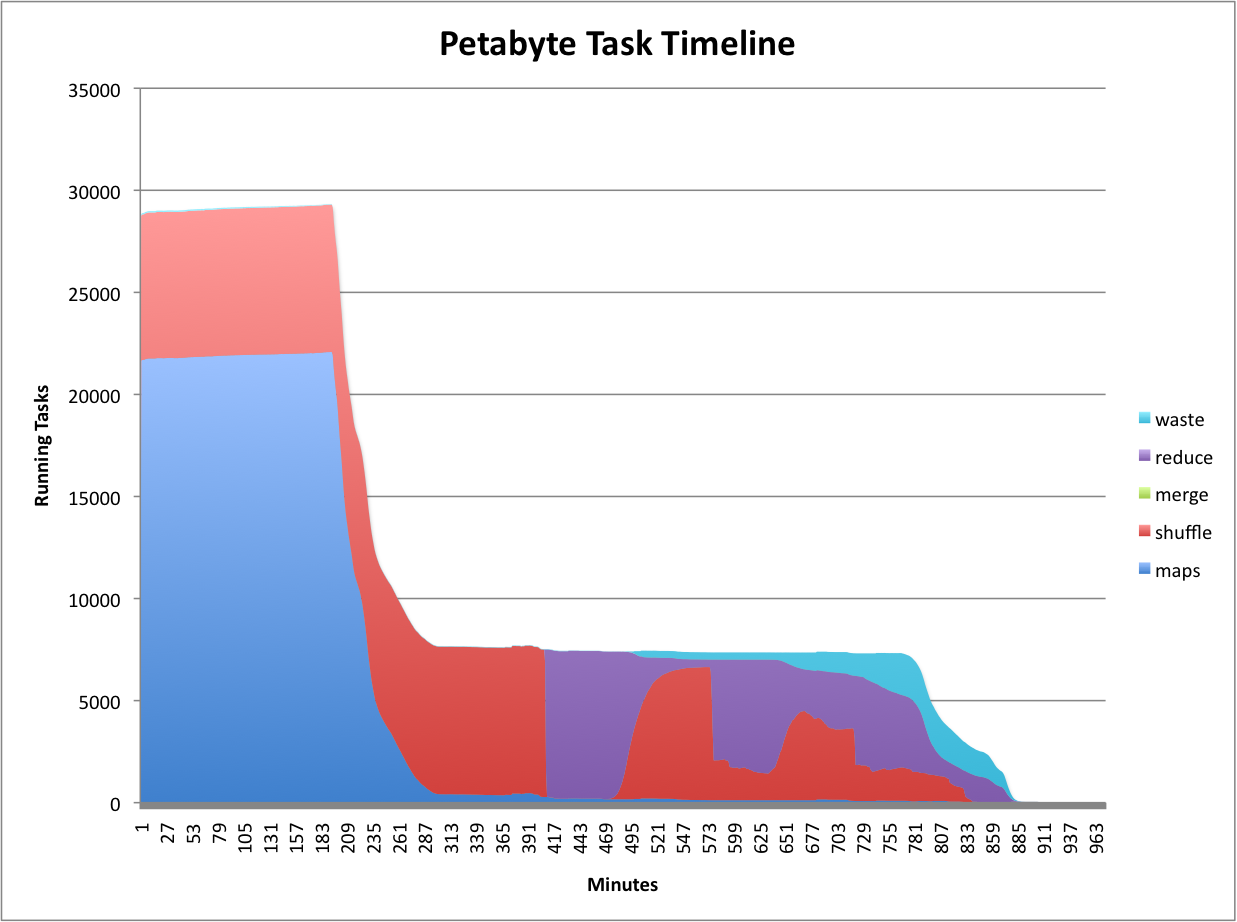
\includegraphics[width=4.5in]{1PBTaskTime.png}
\caption{1 PB sort tasks across time}\label{1PbTimeline}
\end{figure} 

\end{document}
